\documentclass[11pt]{beamer}
%\documentclass[handout,10pt]{beamer}


\usetheme{Copenhagen}


%\usepackage{url}
\usepackage[german]{babel}
\usepackage[latin1]{inputenc}
% \usepackage{booktabs}			% Formatierung der Tabellen
% \usepackage{dcolumn}			% Ausrichtung der Tabellenzelleninhalte
% \usepackage{bm}						% Fettschrift im mathmode
% \usepackage{subfigure}
\usepackage{color}
\usepackage{booktabs}
% *.eps & PSTricks in pdf nutzen
%\usepackage{epstopdf}	% Aus eps Dateien pdf Dateien erzeugen

% Erzeugung der ps / pdf Dateien aus PSTricks Grafiken:
% 1x mit LaTeX => pdf kompilieren
% 1x mit ps2pdf kompilieren
% 1x mit LaTeX => pdf kompilieren
%\usepackage{pst-pdf}		

%Handzettel erstellen?
%\usepackage{pgfpages}
%\only<handout>{\pgfpagesuselayout{4 on 1}[a4paper,border shrink=5mm]}

% oder was auch immer


\usepackage{listings}

%\lstset{tabsize=2,basicstyle=\small\rmfamily,language=java}
\definecolor{lbcolor}{rgb}{0.95,0.95,0.95}



% \newcommand{\RR}[1]{\mathbb R\raisebox{1.1ex}{\scriptsize $#1$}}

\title[]{Domain-specific Performance Optimizations\\ of Pattern Matching in Henshin}
\author[]{Timo Kehrer, Manuel Ohrndorf}
\institute[]{
  Software Engineering Group\\
  Univ. of Siegen}
\date{``Henshin Monthly''\\ \today}


\setbeamercovered{transparent}


\begin{document}

% Mit Hintergrundbild auf Titel-Frame
% {\usebackgroundtemplate{\includegraphics[scale=.55]{graphics/background}}%[viewport=0 0 72 72]\hspace{5cm}
% \begin{frame}
%   \titlepage
% \end{frame}}

% Ohne Hintergrundbild auf Titel-Frame
\frame[plain]{\titlepage}





% \begin{frame}
%  \tableofcontents
%  % Die Option [pausesections] k�nnte n�tzlich sein.
% \end{frame}


\section{Application Domain}

\begin{frame}<beamer>
   \tableofcontents[currentsection]
\end{frame}


\begin{frame}{Meta-model (Representation of Model Differences)}
  \begin{figure}
    \vspace{-0.8cm}
    \hspace*{-1cm}
    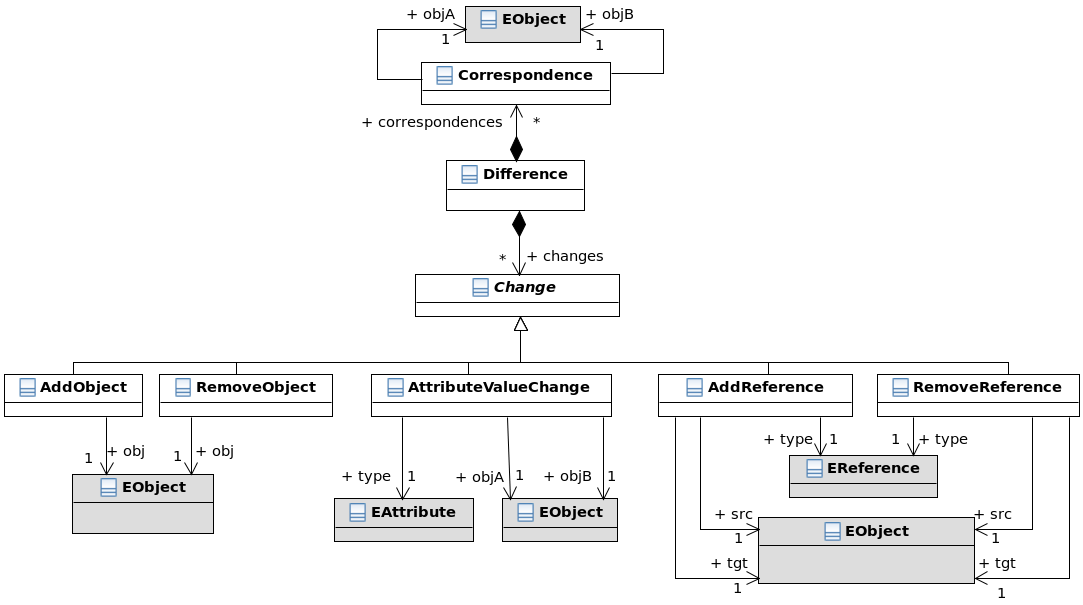
\includegraphics[width=1.15\textwidth]{pic/diffmodel-reduced.png}
  \end{figure}
\end{frame}





\begin{frame}{Change Set Recognition Rules}
  \begin{itemize}
   \item Example: ``Restrict association navigability'' in UML (clipping)
   \item We use Henshin as pattern matching engine for detecting such change patterns
   \item Involved changes are finally grouped to so called semantic change sets
  \end{itemize}

  \begin{figure}
  \vspace{-0.8cm}
  \hspace*{-0.9cm}
  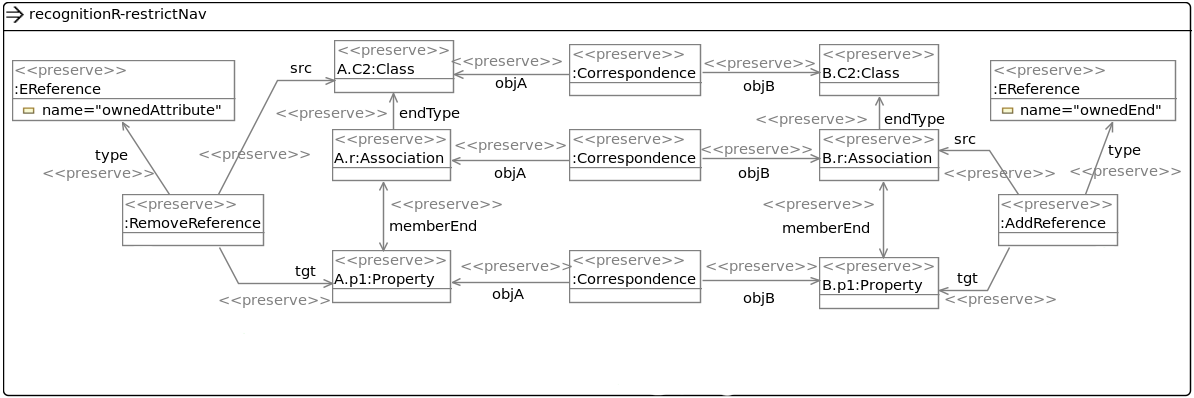
\includegraphics[width=1.15\textwidth]{pic/detect-setAssNav.png}
  \end{figure}
\end{frame}


\begin{frame}{Recognition of Semantic Change Sets}
Problem description: 
\begin{itemize}
\item Given a rule set R and a difference D (``difference model'')
\item For each rule r in R, find all matches in D 
\end{itemize}

\bigskip
Assumptions:
\begin{itemize}
  \item None of the rules in R modifies our model D, i.e. all rules are parallel independent of each other
  \item The rule set R is fixed and none of the rules is modified at runtime 
\end{itemize} 
\end{frame}




\section{Performance Optimizations}

\begin{frame}<beamer>
   \tableofcontents[currentsection]
\end{frame}


\begin{frame}{Overview}
\begin{itemize}
  \item Parallel execution with a pool of worker threads
  \medskip
  \item Sorting of LHS nodes
  \medskip
  \item Reduction of the pre-defined rule set 
  \medskip
  \item Creation of minimal EGraphs 
\end{itemize}
\end{frame}


\begin{frame}{Sorting of LHS Nodes}
Two (in general orthogonal) heuristics:
\begin{itemize}
\item Number of occurrences of objects of a certain type in a difference
\item ``Position'' of LHS nodes within a rule 
\end{itemize}

\bigskip

Remarks:
\begin{itemize}
\item Sorting determines the order in which the recursive constraint solving algorithm locks variables
\item Heuristics similar to generic heuristics in Henshin matching engine? 
\end{itemize} 
\end{frame}



\begin{frame}{Reduction of the Pre-defined Rule Set}
Basic proceeding:
\begin{enumerate}

\item Create index on difference D: 
\begin{itemize}
\item  EClass $\rightarrow$ int, t $\mapsto NoN_t^M$ 
\item  $NoN_t^M$ is the number of objects of type t (or one of its subtypes) in D 
\end{itemize}

\item Create index (``signature'') for each rule r in R
\begin{itemize}
\item  EClass $\rightarrow$ int, t $\mapsto NoN_t^R$ 
\item  $NoN_t^R$ is the number of objects of type t in R 
\end{itemize}
 
\item A rule is matchable if its signature can be found in D

\end{enumerate}

\bigskip
Extensions:
\begin{itemize}
\item Basic proceeding is extended to domain-specific type definitions
\item For instance, tuples such as (AddObject,obj) or (AddReference,src,tgt,type) can be regarded as complex types 
\end{itemize}

\end{frame}



\begin{frame}{Creation of Minimal EGraphs}
Basic idea: 
\begin{itemize}
\item  We create a separate EGraph for finding all matches of a rule. 
\end{itemize}

\medskip

General proceeding:
\begin{itemize}
\item Given a rule r, let $T_r$ be the set of all node types used by r
\item EGraph G = \{o $\in$ D $\vert$ (o.type $\in$ $T_r$) $\lor$ \\ 
 \ \ \ \ \ \ \ \ \ \ \ \ \ \ \ \ \ \ \ \ \ \ \ \ \ \ \ \ \ (o.type.allSuperTypes $\cap T_r \neq \emptyset$)\} 
\end{itemize}

\bigskip

Remarks:
\begin{itemize}
\item Should be already handled by reducing the CSP solution space based on type constraints
\item However, basic proceeding is extended to domain-specific definitions of complex types  
\end{itemize}


\end{frame}





\section{Experiences and Conclusions}

\begin{frame}<beamer>
   \tableofcontents[currentsection]
\end{frame}


\begin{frame}{Experiences and Conclusions}
  \begin{itemize}
   
   \item \textbf{Parallel execution:}
   \begin{itemize}
    \item Strongly depends on the underlying hardware 
   \end{itemize}
   \medskip

   \item \textbf{Sorting of LHS nodes:}
   \begin{itemize}
    \item Biggest performance gain, even for very small models (from minutes to seconds)
    \item Should now already be handled by generic sorting of CSP variables
   \end{itemize}
   \medskip

   \item \textbf{Rule set reduction:}
   \begin{itemize}
    \item Moderate performance gain for large rule sets ($>$ 500 rules)
    \item Generalizable, but current rule set has to be continuously adapted 
   \end{itemize}
   \medskip
   
   \item \textbf{Minimal EGraphs:}
   \begin{itemize}
    \item Similar to reducing the CSP solution space based on type constraints 
    \item Generalization option: API or config file for application-specific definitions of complex types
   \end{itemize}
      
  \end{itemize}
\end{frame}


\end{document}
